\documentclass[1p]{elsarticle_modified}
%\bibliographystyle{elsarticle-num}

%\usepackage[colorlinks]{hyperref}
%\usepackage{abbrmath_seonhwa} %\Abb, \Ascr, \Acal ,\Abf, \Afrak
\usepackage{amsfonts}
\usepackage{amssymb}
\usepackage{amsmath}
\usepackage{amsthm}
\usepackage{scalefnt}
\usepackage{amsbsy}
\usepackage{kotex}
\usepackage{caption}
\usepackage{subfig}
\usepackage{color}
\usepackage{graphicx}
\usepackage{xcolor} %% white, black, red, green, blue, cyan, magenta, yellow
\usepackage{float}
\usepackage{setspace}
\usepackage{hyperref}

\usepackage{tikz}
\usetikzlibrary{arrows}

\usepackage{multirow}
\usepackage{array} % fixed length table
\usepackage{hhline}

%%%%%%%%%%%%%%%%%%%%%
\makeatletter
\renewcommand*\env@matrix[1][\arraystretch]{%
	\edef\arraystretch{#1}%
	\hskip -\arraycolsep
	\let\@ifnextchar\new@ifnextchar
	\array{*\c@MaxMatrixCols c}}
\makeatother %https://tex.stackexchange.com/questions/14071/how-can-i-increase-the-line-spacing-in-a-matrix
%%%%%%%%%%%%%%%

\usepackage[normalem]{ulem}

\newcommand{\msout}[1]{\ifmmode\text{\sout{\ensuremath{#1}}}\else\sout{#1}\fi}
%SOURCE: \msout is \stkout macro in https://tex.stackexchange.com/questions/20609/strikeout-in-math-mode

\newcommand{\cancel}[1]{
	\ifmmode
	{\color{red}\msout{#1}}
	\else
	{\color{red}\sout{#1}}
	\fi
}

\newcommand{\add}[1]{
	{\color{blue}\uwave{#1}}
}

\newcommand{\replace}[2]{
	\ifmmode
	{\color{red}\msout{#1}}{\color{blue}\uwave{#2}}
	\else
	{\color{red}\sout{#1}}{\color{blue}\uwave{#2}}
	\fi
}

\newcommand{\Sol}{\mathcal{S}} %segment
\newcommand{\D}{D} %diagram
\newcommand{\A}{\mathcal{A}} %arc


%%%%%%%%%%%%%%%%%%%%%%%%%%%%%5 test

\def\sl{\operatorname{\textup{SL}}(2,\Cbb)}
\def\psl{\operatorname{\textup{PSL}}(2,\Cbb)}
\def\quan{\mkern 1mu \triangleright \mkern 1mu}

\theoremstyle{definition}
\newtheorem{thm}{Theorem}[section]
\newtheorem{prop}[thm]{Proposition}
\newtheorem{lem}[thm]{Lemma}
\newtheorem{ques}[thm]{Question}
\newtheorem{cor}[thm]{Corollary}
\newtheorem{defn}[thm]{Definition}
\newtheorem{exam}[thm]{Example}
\newtheorem{rmk}[thm]{Remark}
\newtheorem{alg}[thm]{Algorithm}

\newcommand{\I}{\sqrt{-1}}
\begin{document}

%\begin{frontmatter}
%
%\title{Boundary parabolic representations of knots up to 8 crossings}
%
%%% Group authors per affiliation:
%\author{Yunhi Cho} 
%\address{Department of Mathematics, University of Seoul, Seoul, Korea}
%\ead{yhcho@uos.ac.kr}
%
%
%\author{Seonhwa Kim} %\fnref{s_kim}}
%\address{Center for Geometry and Physics, Institute for Basic Science, Pohang, 37673, Korea}
%\ead{ryeona17@ibs.re.kr}
%
%\author{Hyuk Kim}
%\address{Department of Mathematical Sciences, Seoul National University, Seoul 08826, Korea}
%\ead{hyukkim@snu.ac.kr}
%
%\author{Seokbeom Yoon}
%\address{Department of Mathematical Sciences, Seoul National University, Seoul, 08826,  Korea}
%\ead{sbyoon15@snu.ac.kr}
%
%\begin{abstract}
%We find all boundary parabolic representation of knots up to 8 crossings.
%
%\end{abstract}
%\begin{keyword}
%    \MSC[2010] 57M25 
%\end{keyword}
%
%\end{frontmatter}

%\linenumbers
%\tableofcontents
%
\newcommand\colored[1]{\textcolor{white}{\rule[-0.35ex]{0.8em}{1.4ex}}\kern-0.8em\color{red} #1}%
%\newcommand\colored[1]{\textcolor{white}{ #1}\kern-2.17ex	\textcolor{white}{ #1}\kern-1.81ex	\textcolor{white}{ #1}\kern-2.15ex\color{red}#1	}

{\Large $\underline{12n_{0736}~(K12n_{0736})}$}

\setlength{\tabcolsep}{10pt}
\renewcommand{\arraystretch}{1.6}
\vspace{1cm}\begin{tabular}{m{100pt}>{\centering\arraybackslash}m{274pt}}
\multirow{5}{120pt}{
	\centering
	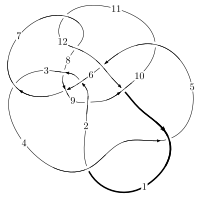
\includegraphics[width=112pt]{../../../GIT/diagram.site/Diagrams/png/2825_12n_0736.png}\\
\ \ \ A knot diagram\footnotemark}&
\allowdisplaybreaks
\textbf{Linearized knot diagam} \\
\cline{2-2}
 &
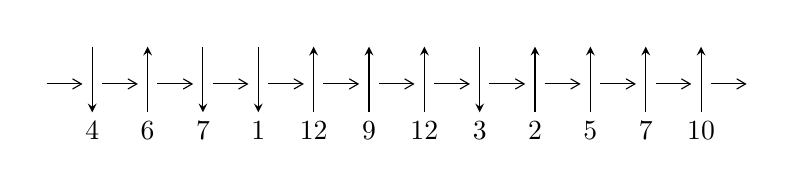
\begin{tikzpicture}[x=20pt, y=17pt]
	% nodes
	\node (C0) at (0, 0) {};
	\node (C1) at (1, 0) {};
	\node (C1U) at (1, +1) {};
	\node (C1D) at (1, -1) {4};

	\node (C2) at (2, 0) {};
	\node (C2U) at (2, +1) {};
	\node (C2D) at (2, -1) {6};

	\node (C3) at (3, 0) {};
	\node (C3U) at (3, +1) {};
	\node (C3D) at (3, -1) {7};

	\node (C4) at (4, 0) {};
	\node (C4U) at (4, +1) {};
	\node (C4D) at (4, -1) {1};

	\node (C5) at (5, 0) {};
	\node (C5U) at (5, +1) {};
	\node (C5D) at (5, -1) {12};

	\node (C6) at (6, 0) {};
	\node (C6U) at (6, +1) {};
	\node (C6D) at (6, -1) {9};

	\node (C7) at (7, 0) {};
	\node (C7U) at (7, +1) {};
	\node (C7D) at (7, -1) {12};

	\node (C8) at (8, 0) {};
	\node (C8U) at (8, +1) {};
	\node (C8D) at (8, -1) {3};

	\node (C9) at (9, 0) {};
	\node (C9U) at (9, +1) {};
	\node (C9D) at (9, -1) {2};

	\node (C10) at (10, 0) {};
	\node (C10U) at (10, +1) {};
	\node (C10D) at (10, -1) {5};

	\node (C11) at (11, 0) {};
	\node (C11U) at (11, +1) {};
	\node (C11D) at (11, -1) {7};

	\node (C12) at (12, 0) {};
	\node (C12U) at (12, +1) {};
	\node (C12D) at (12, -1) {10};
	\node (C13) at (13, 0) {};

	% arrows
	\draw[->,>={angle 60}]
	(C0) edge (C1) (C1) edge (C2) (C2) edge (C3) (C3) edge (C4) (C4) edge (C5) (C5) edge (C6) (C6) edge (C7) (C7) edge (C8) (C8) edge (C9) (C9) edge (C10) (C10) edge (C11) (C11) edge (C12) (C12) edge (C13) ;	\draw[->,>=stealth]
	(C1U) edge (C1D) (C2D) edge (C2U) (C3U) edge (C3D) (C4U) edge (C4D) (C5D) edge (C5U) (C6D) edge (C6U) (C7D) edge (C7U) (C8U) edge (C8D) (C9D) edge (C9U) (C10D) edge (C10U) (C11D) edge (C11U) (C12D) edge (C12U) ;
	\end{tikzpicture} \\
\hhline{~~} \\& 
\textbf{Solving Sequence} \\ \cline{2-2} 
 &
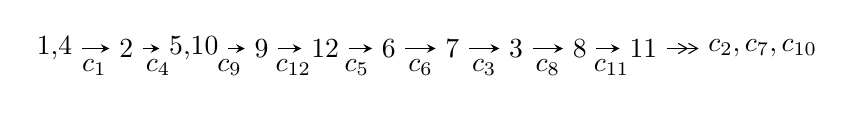
\begin{tikzpicture}[x=23pt, y=7pt]
	% node
	\node (A0) at (-1/8, 0) {1,4};
	\node (A1) at (1, 0) {2};
	\node (A2) at (33/16, 0) {5,10};
	\node (A3) at (25/8, 0) {9};
	\node (A4) at (33/8, 0) {12};
	\node (A5) at (41/8, 0) {6};
	\node (A6) at (49/8, 0) {7};
	\node (A7) at (57/8, 0) {3};
	\node (A8) at (65/8, 0) {8};
	\node (A9) at (73/8, 0) {11};
	\node (C1) at (1/2, -1) {$c_{1}$};
	\node (C2) at (3/2, -1) {$c_{4}$};
	\node (C3) at (21/8, -1) {$c_{9}$};
	\node (C4) at (29/8, -1) {$c_{12}$};
	\node (C5) at (37/8, -1) {$c_{5}$};
	\node (C6) at (45/8, -1) {$c_{6}$};
	\node (C7) at (53/8, -1) {$c_{3}$};
	\node (C8) at (61/8, -1) {$c_{8}$};
	\node (C9) at (69/8, -1) {$c_{11}$};
	\node (A10) at (11, 0) {$c_{2},c_{7},c_{10}$};

	% edge
	\draw[->,>=stealth]	
	(A0) edge (A1) (A1) edge (A2) (A2) edge (A3) (A3) edge (A4) (A4) edge (A5) (A5) edge (A6) (A6) edge (A7) (A7) edge (A8) (A8) edge (A9) ;
	\draw[->>,>={angle 60}]	
	(A9) edge (A10);
\end{tikzpicture} \\ 

\end{tabular} \\

\footnotetext{
The image of knot diagram is generated by the software ``\textbf{Draw programme}" developed by Andrew Bartholomew(\url{http://www.layer8.co.uk/maths/draw/index.htm\#Running-draw}), where we modified some parts for our purpose(\url{https://github.com/CATsTAILs/LinksPainter}).
}\phantom \\ \newline 
\centering \textbf{Ideals for irreducible components\footnotemark of $X_{\text{par}}$} 
 
\begin{align*}
I^u_{1}&=\langle 
6.85974\times10^{510} u^{118}-3.36065\times10^{511} u^{117}+\cdots+8.39335\times10^{511} b-2.36017\times10^{513},\\
\phantom{I^u_{1}}&\phantom{= \langle  }-8.34995\times10^{512} u^{118}-7.74279\times10^{513} u^{117}+\cdots+1.02315\times10^{515} a+2.17745\times10^{517},\\
\phantom{I^u_{1}}&\phantom{= \langle  }u^{119}-5 u^{118}+\cdots+33731 u-1219\rangle \\
I^u_{2}&=\langle 
-5.01803\times10^{47} u^{43}+5.12787\times10^{48} u^{42}+\cdots+8.93849\times10^{46} b+4.54183\times10^{46},\\
\phantom{I^u_{2}}&\phantom{= \langle  }4.44342\times10^{47} u^{43}-4.47435\times10^{48} u^{42}+\cdots+8.93849\times10^{46} a-1.52859\times10^{48},\;u^{44}-10 u^{43}+\cdots-19 u+1\rangle \\
\\
\end{align*}
\raggedright * 2 irreducible components of $\dim_{\mathbb{C}}=0$, with total 163 representations.\\
\footnotetext{All coefficients of polynomials are rational numbers. But the coefficients are sometimes approximated in decimal forms when there is not enough margin.}
\newpage
\renewcommand{\arraystretch}{1}
\centering \section*{I. $I^u_{1}= \langle 6.86\times10^{510} u^{118}-3.36\times10^{511} u^{117}+\cdots+8.39\times10^{511} b-2.36\times10^{513},\;-8.35\times10^{512} u^{118}-7.74\times10^{513} u^{117}+\cdots+1.02\times10^{515} a+2.18\times10^{517},\;u^{119}-5 u^{118}+\cdots+33731 u-1219 \rangle$}
\flushleft \textbf{(i) Arc colorings}\\
\begin{tabular}{m{7pt} m{180pt} m{7pt} m{180pt} }
\flushright $a_{1}=$&$\begin{pmatrix}1\\0\end{pmatrix}$ \\
\flushright $a_{4}=$&$\begin{pmatrix}0\\u\end{pmatrix}$ \\
\flushright $a_{2}=$&$\begin{pmatrix}1\\u^2\end{pmatrix}$ \\
\flushright $a_{5}=$&$\begin{pmatrix}- u\\u\end{pmatrix}$ \\
\flushright $a_{10}=$&$\begin{pmatrix}0.00816103 u^{118}+0.0756760 u^{117}+\cdots+5478.41 u-212.818\\-0.0817283 u^{118}+0.400395 u^{117}+\cdots-616.990 u+28.1195\end{pmatrix}$ \\
\flushright $a_{9}=$&$\begin{pmatrix}0.0879763 u^{118}-0.404797 u^{117}+\cdots+2176.32 u-98.9470\\-0.138109 u^{118}+0.752524 u^{117}+\cdots+2225.89 u-71.1027\end{pmatrix}$ \\
\flushright $a_{12}=$&$\begin{pmatrix}-0.0959043 u^{118}+0.466145 u^{117}+\cdots-953.729 u+29.7923\\0.0946342 u^{118}-0.487040 u^{117}+\cdots-534.337 u+15.0636\end{pmatrix}$ \\
\flushright $a_{6}=$&$\begin{pmatrix}0.103143 u^{118}-0.603357 u^{117}+\cdots-3937.06 u+141.473\\-0.0286967 u^{118}+0.253557 u^{117}+\cdots+4653.40 u-167.154\end{pmatrix}$ \\
\flushright $a_{7}=$&$\begin{pmatrix}0.0414577 u^{118}-0.290467 u^{117}+\cdots-3968.39 u+147.548\\0.0852643 u^{118}-0.410546 u^{117}+\cdots+662.359 u-30.1911\end{pmatrix}$ \\
\flushright $a_{3}=$&$\begin{pmatrix}0.0419752 u^{118}-0.130654 u^{117}+\cdots+3960.26 u-143.179\\-0.130629 u^{118}+0.664912 u^{117}+\cdots+213.624 u-0.0470890\end{pmatrix}$ \\
\flushright $a_{8}=$&$\begin{pmatrix}-0.0129848 u^{118}+0.210555 u^{117}+\cdots+7096.23 u-266.439\\-0.163462 u^{118}+0.770953 u^{117}+\cdots-2622.80 u+104.586\end{pmatrix}$ \\
\flushright $a_{11}=$&$\begin{pmatrix}0.0621343 u^{118}-0.282625 u^{117}+\cdots+1737.87 u-80.8801\\-0.135702 u^{118}+0.758695 u^{117}+\cdots+3123.55 u-103.818\end{pmatrix}$\\&\end{tabular}
\flushleft \textbf{(ii) Obstruction class $= -1$}\\~\\
\flushleft \textbf{(iii) Cusp Shapes $= -0.171027 u^{118}+0.892492 u^{117}+\cdots+742.503 u-13.0567$}\\~\\
\newpage\renewcommand{\arraystretch}{1}
\flushleft \textbf{(iv) u-Polynomials at the component}\newline \\
\begin{tabular}{m{50pt}|m{274pt}}
Crossings & \hspace{64pt}u-Polynomials at each crossing \\
\hline $$\begin{aligned}c_{1},c_{4}\end{aligned}$$&$\begin{aligned}
&u^{119}+5 u^{118}+\cdots+33731 u+1219
\end{aligned}$\\
\hline $$\begin{aligned}c_{2}\end{aligned}$$&$\begin{aligned}
&u^{119}-8 u^{118}+\cdots-4 u-1
\end{aligned}$\\
\hline $$\begin{aligned}c_{3}\end{aligned}$$&$\begin{aligned}
&u^{119}-14 u^{117}+\cdots+152947565649 u-9784213871
\end{aligned}$\\
\hline $$\begin{aligned}c_{5}\end{aligned}$$&$\begin{aligned}
&u^{119}+2 u^{118}+\cdots+2467110921 u-1915307993
\end{aligned}$\\
\hline $$\begin{aligned}c_{6}\end{aligned}$$&$\begin{aligned}
&u^{119}+4 u^{118}+\cdots+6 u-1
\end{aligned}$\\
\hline $$\begin{aligned}c_{7},c_{11}\end{aligned}$$&$\begin{aligned}
&u^{119}-3 u^{118}+\cdots-2145918 u-358027
\end{aligned}$\\
\hline $$\begin{aligned}c_{8}\end{aligned}$$&$\begin{aligned}
&u^{119}- u^{118}+\cdots-2803281 u-360061
\end{aligned}$\\
\hline $$\begin{aligned}c_{9}\end{aligned}$$&$\begin{aligned}
&u^{119}-4 u^{118}+\cdots-2405770 u-8033011
\end{aligned}$\\
\hline $$\begin{aligned}c_{10}\end{aligned}$$&$\begin{aligned}
&u^{119}- u^{118}+\cdots-40925 u-4771
\end{aligned}$\\
\hline $$\begin{aligned}c_{12}\end{aligned}$$&$\begin{aligned}
&u^{119}+7 u^{118}+\cdots-26 u-1
\end{aligned}$\\
\hline
\end{tabular}\\~\\
\newpage\renewcommand{\arraystretch}{1}
\flushleft \textbf{(v) Riley Polynomials at the component}\newline \\
\begin{tabular}{m{50pt}|m{274pt}}
Crossings & \hspace{64pt}Riley Polynomials at each crossing \\
\hline $$\begin{aligned}c_{1},c_{4}\end{aligned}$$&$\begin{aligned}
&y^{119}+71 y^{118}+\cdots+441068225 y-1485961
\end{aligned}$\\
\hline $$\begin{aligned}c_{2}\end{aligned}$$&$\begin{aligned}
&y^{119}+38 y^{118}+\cdots-296 y-1
\end{aligned}$\\
\hline $$\begin{aligned}c_{3}\end{aligned}$$&$\begin{aligned}
&y^{119}-28 y^{118}+\cdots+4.07\times10^{21} y-9.57\times10^{19}
\end{aligned}$\\
\hline $$\begin{aligned}c_{5}\end{aligned}$$&$\begin{aligned}
&y^{119}+54 y^{118}+\cdots-4.20\times10^{19} y-3.67\times10^{18}
\end{aligned}$\\
\hline $$\begin{aligned}c_{6}\end{aligned}$$&$\begin{aligned}
&y^{119}-14 y^{118}+\cdots-2 y-1
\end{aligned}$\\
\hline $$\begin{aligned}c_{7},c_{11}\end{aligned}$$&$\begin{aligned}
&y^{119}+87 y^{118}+\cdots-6209933896494 y-128183332729
\end{aligned}$\\
\hline $$\begin{aligned}c_{8}\end{aligned}$$&$\begin{aligned}
&y^{119}-37 y^{118}+\cdots+387766004639 y-129643923721
\end{aligned}$\\
\hline $$\begin{aligned}c_{9}\end{aligned}$$&$\begin{aligned}
&y^{119}+48 y^{118}+\cdots-3572692300957120 y-64529265726121
\end{aligned}$\\
\hline $$\begin{aligned}c_{10}\end{aligned}$$&$\begin{aligned}
&y^{119}+13 y^{118}+\cdots-5029200903 y-22762441
\end{aligned}$\\
\hline $$\begin{aligned}c_{12}\end{aligned}$$&$\begin{aligned}
&y^{119}-25 y^{118}+\cdots+172 y-1
\end{aligned}$\\
\hline
\end{tabular}\\~\\
\newpage\flushleft \textbf{(vi) Complex Volumes and Cusp Shapes}
$$\begin{array}{c|c|c}  
\text{Solutions to }I^u_{1}& \I (\text{vol} + \sqrt{-1}CS) & \text{Cusp shape}\\
 \hline 
\begin{aligned}
u &= \phantom{-}0.900710 + 0.447742 I \\
a &= \phantom{-}1.32134 + 0.75592 I \\
b &= -1.080900 + 0.694050 I\end{aligned}
 & -6.44500 - 4.63461 I & \phantom{-0.000000 } 0 \\ \hline\begin{aligned}
u &= \phantom{-}0.900710 - 0.447742 I \\
a &= \phantom{-}1.32134 - 0.75592 I \\
b &= -1.080900 - 0.694050 I\end{aligned}
 & -6.44500 + 4.63461 I & \phantom{-0.000000 } 0 \\ \hline\begin{aligned}
u &= -0.449046 + 0.880282 I \\
a &= \phantom{-}0.334901 - 0.759799 I \\
b &= -0.89030 + 1.41189 I\end{aligned}
 & -6.27923 + 2.06623 I & \phantom{-0.000000 } 0 \\ \hline\begin{aligned}
u &= -0.449046 - 0.880282 I \\
a &= \phantom{-}0.334901 + 0.759799 I \\
b &= -0.89030 - 1.41189 I\end{aligned}
 & -6.27923 - 2.06623 I & \phantom{-0.000000 } 0 \\ \hline\begin{aligned}
u &= -0.427914 + 0.885888 I \\
a &= -0.169526 - 1.068510 I \\
b &= \phantom{-}0.161027 - 1.059390 I\end{aligned}
 & -5.95151 - 4.58997 I & \phantom{-0.000000 } 0 \\ \hline\begin{aligned}
u &= -0.427914 - 0.885888 I \\
a &= -0.169526 + 1.068510 I \\
b &= \phantom{-}0.161027 + 1.059390 I\end{aligned}
 & -5.95151 + 4.58997 I & \phantom{-0.000000 } 0 \\ \hline\begin{aligned}
u &= \phantom{-}0.316551 + 0.968693 I \\
a &= -1.88014 - 0.69352 I \\
b &= \phantom{-}1.69695 - 0.11936 I\end{aligned}
 & \phantom{-}5.80304 - 1.31943 I & \phantom{-0.000000 } 0 \\ \hline\begin{aligned}
u &= \phantom{-}0.316551 - 0.968693 I \\
a &= -1.88014 + 0.69352 I \\
b &= \phantom{-}1.69695 + 0.11936 I\end{aligned}
 & \phantom{-}5.80304 + 1.31943 I & \phantom{-0.000000 } 0 \\ \hline\begin{aligned}
u &= \phantom{-}0.088614 + 0.967014 I \\
a &= \phantom{-}1.11936 + 2.02388 I \\
b &= -0.1003180 + 0.0011885 I\end{aligned}
 & \phantom{-}2.64569 + 0.92590 I & \phantom{-0.000000 } 0 \\ \hline\begin{aligned}
u &= \phantom{-}0.088614 - 0.967014 I \\
a &= \phantom{-}1.11936 - 2.02388 I \\
b &= -0.1003180 - 0.0011885 I\end{aligned}
 & \phantom{-}2.64569 - 0.92590 I & \phantom{-0.000000 } 0\\
 \hline 
 \end{array}$$\newpage$$\begin{array}{c|c|c}  
\text{Solutions to }I^u_{1}& \I (\text{vol} + \sqrt{-1}CS) & \text{Cusp shape}\\
 \hline 
\begin{aligned}
u &= \phantom{-}0.034600 + 0.968501 I \\
a &= -3.18293 + 0.17058 I \\
b &= \phantom{-}2.75536 + 0.20472 I\end{aligned}
 & \phantom{-}8.19227 - 0.15281 I & \phantom{-0.000000 } 0 \\ \hline\begin{aligned}
u &= \phantom{-}0.034600 - 0.968501 I \\
a &= -3.18293 - 0.17058 I \\
b &= \phantom{-}2.75536 - 0.20472 I\end{aligned}
 & \phantom{-}8.19227 + 0.15281 I & \phantom{-0.000000 } 0 \\ \hline\begin{aligned}
u &= \phantom{-}0.468693 + 0.931901 I \\
a &= \phantom{-}0.874360 - 0.125803 I \\
b &= -0.370722 + 0.380148 I\end{aligned}
 & -0.68578 - 2.05545 I & \phantom{-0.000000 } 0 \\ \hline\begin{aligned}
u &= \phantom{-}0.468693 - 0.931901 I \\
a &= \phantom{-}0.874360 + 0.125803 I \\
b &= -0.370722 - 0.380148 I\end{aligned}
 & -0.68578 + 2.05545 I & \phantom{-0.000000 } 0 \\ \hline\begin{aligned}
u &= \phantom{-}0.524053 + 0.903789 I \\
a &= \phantom{-}0.429339 + 0.831533 I \\
b &= -0.397239 + 0.978211 I\end{aligned}
 & -4.22261 - 5.62713 I & \phantom{-0.000000 } 0 \\ \hline\begin{aligned}
u &= \phantom{-}0.524053 - 0.903789 I \\
a &= \phantom{-}0.429339 - 0.831533 I \\
b &= -0.397239 - 0.978211 I\end{aligned}
 & -4.22261 + 5.62713 I & \phantom{-0.000000 } 0 \\ \hline\begin{aligned}
u &= \phantom{-}0.942515 + 0.466420 I \\
a &= \phantom{-}0.0687464 - 0.0524007 I \\
b &= \phantom{-}0.421089 - 0.836959 I\end{aligned}
 & -1.95977 - 3.15258 I & \phantom{-0.000000 } 0 \\ \hline\begin{aligned}
u &= \phantom{-}0.942515 - 0.466420 I \\
a &= \phantom{-}0.0687464 + 0.0524007 I \\
b &= \phantom{-}0.421089 + 0.836959 I\end{aligned}
 & -1.95977 + 3.15258 I & \phantom{-0.000000 } 0 \\ \hline\begin{aligned}
u &= -0.912733 + 0.534874 I \\
a &= \phantom{-}0.387490 - 0.015209 I \\
b &= -0.344925 - 0.072303 I\end{aligned}
 & \phantom{-}0.62504 - 2.59860 I & \phantom{-0.000000 } 0 \\ \hline\begin{aligned}
u &= -0.912733 - 0.534874 I \\
a &= \phantom{-}0.387490 + 0.015209 I \\
b &= -0.344925 + 0.072303 I\end{aligned}
 & \phantom{-}0.62504 + 2.59860 I & \phantom{-0.000000 } 0\\
 \hline 
 \end{array}$$\newpage$$\begin{array}{c|c|c}  
\text{Solutions to }I^u_{1}& \I (\text{vol} + \sqrt{-1}CS) & \text{Cusp shape}\\
 \hline 
\begin{aligned}
u &= -0.351789 + 1.000600 I \\
a &= \phantom{-}0.342892 - 0.392805 I \\
b &= -0.015754 - 1.316610 I\end{aligned}
 & -5.37643 + 2.67841 I & \phantom{-0.000000 } 0 \\ \hline\begin{aligned}
u &= -0.351789 - 1.000600 I \\
a &= \phantom{-}0.342892 + 0.392805 I \\
b &= -0.015754 + 1.316610 I\end{aligned}
 & -5.37643 - 2.67841 I & \phantom{-0.000000 } 0 \\ \hline\begin{aligned}
u &= \phantom{-}0.238293 + 1.057470 I \\
a &= -2.38178 - 0.50948 I \\
b &= \phantom{-}0.875887 - 0.130142 I\end{aligned}
 & \phantom{-}3.67325 - 1.82473 I & \phantom{-0.000000 } 0 \\ \hline\begin{aligned}
u &= \phantom{-}0.238293 - 1.057470 I \\
a &= -2.38178 + 0.50948 I \\
b &= \phantom{-}0.875887 + 0.130142 I\end{aligned}
 & \phantom{-}3.67325 + 1.82473 I & \phantom{-0.000000 } 0 \\ \hline\begin{aligned}
u &= -0.533860 + 0.958020 I \\
a &= -1.84072 + 0.15881 I \\
b &= \phantom{-}1.30233 + 1.02834 I\end{aligned}
 & -0.94044 + 2.05443 I & \phantom{-0.000000 } 0 \\ \hline\begin{aligned}
u &= -0.533860 - 0.958020 I \\
a &= -1.84072 - 0.15881 I \\
b &= \phantom{-}1.30233 - 1.02834 I\end{aligned}
 & -0.94044 - 2.05443 I & \phantom{-0.000000 } 0 \\ \hline\begin{aligned}
u &= -0.704256 + 0.552773 I \\
a &= \phantom{-}0.319026 + 0.864267 I \\
b &= \phantom{-}0.612712 - 1.085150 I\end{aligned}
 & -2.11848 + 2.62866 I & \phantom{-0.000000 } 0 \\ \hline\begin{aligned}
u &= -0.704256 - 0.552773 I \\
a &= \phantom{-}0.319026 - 0.864267 I \\
b &= \phantom{-}0.612712 + 1.085150 I\end{aligned}
 & -2.11848 - 2.62866 I & \phantom{-0.000000 } 0 \\ \hline\begin{aligned}
u &= \phantom{-}0.344266 + 1.049950 I \\
a &= -2.41088 + 0.04163 I \\
b &= \phantom{-}1.389530 - 0.046178 I\end{aligned}
 & \phantom{-}3.21889 - 2.43004 I & \phantom{-0.000000 } 0 \\ \hline\begin{aligned}
u &= \phantom{-}0.344266 - 1.049950 I \\
a &= -2.41088 - 0.04163 I \\
b &= \phantom{-}1.389530 + 0.046178 I\end{aligned}
 & \phantom{-}3.21889 + 2.43004 I & \phantom{-0.000000 } 0\\
 \hline 
 \end{array}$$\newpage$$\begin{array}{c|c|c}  
\text{Solutions to }I^u_{1}& \I (\text{vol} + \sqrt{-1}CS) & \text{Cusp shape}\\
 \hline 
\begin{aligned}
u &= -0.005760 + 0.889619 I \\
a &= -1.05334 + 1.09957 I \\
b &= \phantom{-}0.196920 + 0.854551 I\end{aligned}
 & \phantom{-}2.37296 - 1.12400 I & \phantom{-0.000000 } 0 \\ \hline\begin{aligned}
u &= -0.005760 - 0.889619 I \\
a &= -1.05334 - 1.09957 I \\
b &= \phantom{-}0.196920 - 0.854551 I\end{aligned}
 & \phantom{-}2.37296 + 1.12400 I & \phantom{-0.000000 } 0 \\ \hline\begin{aligned}
u &= -0.023932 + 1.113010 I \\
a &= \phantom{-}0.701632 - 0.514535 I \\
b &= -0.815122 + 0.220705 I\end{aligned}
 & -0.57945 - 2.60843 I & \phantom{-0.000000 } 0 \\ \hline\begin{aligned}
u &= -0.023932 - 1.113010 I \\
a &= \phantom{-}0.701632 + 0.514535 I \\
b &= -0.815122 - 0.220705 I\end{aligned}
 & -0.57945 + 2.60843 I & \phantom{-0.000000 } 0 \\ \hline\begin{aligned}
u &= \phantom{-}0.885725 + 0.037717 I \\
a &= \phantom{-}0.416970 + 0.224985 I \\
b &= \phantom{-}0.221133 - 0.730148 I\end{aligned}
 & -2.27128 - 1.04460 I & \phantom{-0.000000 } 0 \\ \hline\begin{aligned}
u &= \phantom{-}0.885725 - 0.037717 I \\
a &= \phantom{-}0.416970 - 0.224985 I \\
b &= \phantom{-}0.221133 + 0.730148 I\end{aligned}
 & -2.27128 + 1.04460 I & \phantom{-0.000000 } 0 \\ \hline\begin{aligned}
u &= -1.028760 + 0.469136 I \\
a &= -0.167751 - 0.361357 I \\
b &= -0.902980 + 0.878633 I\end{aligned}
 & -7.36456 - 4.66244 I & \phantom{-0.000000 } 0 \\ \hline\begin{aligned}
u &= -1.028760 - 0.469136 I \\
a &= -0.167751 + 0.361357 I \\
b &= -0.902980 - 0.878633 I\end{aligned}
 & -7.36456 + 4.66244 I & \phantom{-0.000000 } 0 \\ \hline\begin{aligned}
u &= \phantom{-}0.750537 + 0.421665 I \\
a &= -0.808445 - 0.730052 I \\
b &= -0.468007 - 0.392684 I\end{aligned}
 & -5.46865 + 0.83801 I & \phantom{-0.000000 } 0 \\ \hline\begin{aligned}
u &= \phantom{-}0.750537 - 0.421665 I \\
a &= -0.808445 + 0.730052 I \\
b &= -0.468007 + 0.392684 I\end{aligned}
 & -5.46865 - 0.83801 I & \phantom{-0.000000 } 0\\
 \hline 
 \end{array}$$\newpage$$\begin{array}{c|c|c}  
\text{Solutions to }I^u_{1}& \I (\text{vol} + \sqrt{-1}CS) & \text{Cusp shape}\\
 \hline 
\begin{aligned}
u &= -0.438608 + 1.052740 I \\
a &= \phantom{-}0.776998 - 1.013660 I \\
b &= -1.17427 + 1.51445 I\end{aligned}
 & -5.71211 + 10.11080 I & \phantom{-0.000000 } 0 \\ \hline\begin{aligned}
u &= -0.438608 - 1.052740 I \\
a &= \phantom{-}0.776998 + 1.013660 I \\
b &= -1.17427 - 1.51445 I\end{aligned}
 & -5.71211 - 10.11080 I & \phantom{-0.000000 } 0 \\ \hline\begin{aligned}
u &= -0.028783 + 0.848063 I \\
a &= \phantom{-}2.08400 - 0.54864 I \\
b &= -0.937681 - 0.936397 I\end{aligned}
 & -1.96071 + 2.92636 I & \phantom{-0.000000 } 0 \\ \hline\begin{aligned}
u &= -0.028783 - 0.848063 I \\
a &= \phantom{-}2.08400 + 0.54864 I \\
b &= -0.937681 + 0.936397 I\end{aligned}
 & -1.96071 - 2.92636 I & \phantom{-0.000000 } 0 \\ \hline\begin{aligned}
u &= -0.616411 + 0.972759 I \\
a &= \phantom{-}1.03162 - 0.97316 I \\
b &= -1.49185 - 0.20932 I\end{aligned}
 & \phantom{-}8.63647 + 2.51702 I & \phantom{-0.000000 } 0 \\ \hline\begin{aligned}
u &= -0.616411 - 0.972759 I \\
a &= \phantom{-}1.03162 + 0.97316 I \\
b &= -1.49185 + 0.20932 I\end{aligned}
 & \phantom{-}8.63647 - 2.51702 I & \phantom{-0.000000 } 0 \\ \hline\begin{aligned}
u &= -0.382315 + 0.752935 I \\
a &= \phantom{-}2.95156 - 0.21603 I \\
b &= -1.123000 - 0.742293 I\end{aligned}
 & -6.75118 + 1.52015 I & \phantom{-0.000000 } 0 \\ \hline\begin{aligned}
u &= -0.382315 - 0.752935 I \\
a &= \phantom{-}2.95156 + 0.21603 I \\
b &= -1.123000 + 0.742293 I\end{aligned}
 & -6.75118 - 1.52015 I & \phantom{-0.000000 } 0 \\ \hline\begin{aligned}
u &= -0.285890 + 0.793339 I \\
a &= -3.66741 - 0.67758 I \\
b &= \phantom{-}0.075363 + 0.317107 I\end{aligned}
 & -6.43962 + 7.74698 I & \phantom{-0.000000 } 0 \\ \hline\begin{aligned}
u &= -0.285890 - 0.793339 I \\
a &= -3.66741 + 0.67758 I \\
b &= \phantom{-}0.075363 - 0.317107 I\end{aligned}
 & -6.43962 - 7.74698 I & \phantom{-0.000000 } 0\\
 \hline 
 \end{array}$$\newpage$$\begin{array}{c|c|c}  
\text{Solutions to }I^u_{1}& \I (\text{vol} + \sqrt{-1}CS) & \text{Cusp shape}\\
 \hline 
\begin{aligned}
u &= \phantom{-}0.400440 + 1.113570 I \\
a &= \phantom{-}2.02387 - 0.38423 I \\
b &= -1.42003 + 1.32973 I\end{aligned}
 & -1.08963 - 6.72426 I & \phantom{-0.000000 } 0 \\ \hline\begin{aligned}
u &= \phantom{-}0.400440 - 1.113570 I \\
a &= \phantom{-}2.02387 + 0.38423 I \\
b &= -1.42003 - 1.32973 I\end{aligned}
 & -1.08963 + 6.72426 I & \phantom{-0.000000 } 0 \\ \hline\begin{aligned}
u &= \phantom{-}1.179560 + 0.110814 I \\
a &= -0.176215 - 0.101678 I \\
b &= -0.436606 - 0.909732 I\end{aligned}
 & -7.09503 + 2.33950 I & \phantom{-0.000000 } 0 \\ \hline\begin{aligned}
u &= \phantom{-}1.179560 - 0.110814 I \\
a &= -0.176215 + 0.101678 I \\
b &= -0.436606 + 0.909732 I\end{aligned}
 & -7.09503 - 2.33950 I & \phantom{-0.000000 } 0 \\ \hline\begin{aligned}
u &= -0.158955 + 0.796638 I \\
a &= -0.148100 + 0.022738 I \\
b &= \phantom{-}0.251370 + 1.358570 I\end{aligned}
 & -0.63197 + 5.62831 I & \phantom{-0.000000 } 0 \\ \hline\begin{aligned}
u &= -0.158955 - 0.796638 I \\
a &= -0.148100 - 0.022738 I \\
b &= \phantom{-}0.251370 - 1.358570 I\end{aligned}
 & -0.63197 - 5.62831 I & \phantom{-0.000000 } 0 \\ \hline\begin{aligned}
u &= -0.713990 + 0.333093 I \\
a &= \phantom{-}0.048421 + 0.346386 I \\
b &= \phantom{-}0.755826 - 1.127220 I\end{aligned}
 & -2.66772 - 5.71493 I & \phantom{-0.000000 } 0 \\ \hline\begin{aligned}
u &= -0.713990 - 0.333093 I \\
a &= \phantom{-}0.048421 - 0.346386 I \\
b &= \phantom{-}0.755826 + 1.127220 I\end{aligned}
 & -2.66772 + 5.71493 I & \phantom{-0.000000 } 0 \\ \hline\begin{aligned}
u &= \phantom{-}0.352442 + 1.166840 I \\
a &= \phantom{-}1.271480 - 0.157515 I \\
b &= -0.600113 + 0.145559 I\end{aligned}
 & \phantom{-}1.04936 - 3.15794 I & \phantom{-0.000000 } 0 \\ \hline\begin{aligned}
u &= \phantom{-}0.352442 - 1.166840 I \\
a &= \phantom{-}1.271480 + 0.157515 I \\
b &= -0.600113 - 0.145559 I\end{aligned}
 & \phantom{-}1.04936 + 3.15794 I & \phantom{-0.000000 } 0\\
 \hline 
 \end{array}$$\newpage$$\begin{array}{c|c|c}  
\text{Solutions to }I^u_{1}& \I (\text{vol} + \sqrt{-1}CS) & \text{Cusp shape}\\
 \hline 
\begin{aligned}
u &= -0.554249 + 1.094380 I \\
a &= \phantom{-}0.144098 + 0.597012 I \\
b &= \phantom{-}0.102609 - 0.202619 I\end{aligned}
 & \phantom{-}0.55768 - 2.84906 I & \phantom{-0.000000 } 0 \\ \hline\begin{aligned}
u &= -0.554249 - 1.094380 I \\
a &= \phantom{-}0.144098 - 0.597012 I \\
b &= \phantom{-}0.102609 + 0.202619 I\end{aligned}
 & \phantom{-}0.55768 + 2.84906 I & \phantom{-0.000000 } 0 \\ \hline\begin{aligned}
u &= \phantom{-}1.177440 + 0.384738 I \\
a &= \phantom{-}0.252436 + 0.291822 I \\
b &= \phantom{-}0.248807 - 0.332188 I\end{aligned}
 & -2.71387 - 1.56680 I & \phantom{-0.000000 } 0 \\ \hline\begin{aligned}
u &= \phantom{-}1.177440 - 0.384738 I \\
a &= \phantom{-}0.252436 - 0.291822 I \\
b &= \phantom{-}0.248807 + 0.332188 I\end{aligned}
 & -2.71387 + 1.56680 I & \phantom{-0.000000 } 0 \\ \hline\begin{aligned}
u &= -0.533350 + 1.139550 I \\
a &= -1.95806 + 0.05092 I \\
b &= \phantom{-}1.24441 + 1.02146 I\end{aligned}
 & -0.23770 + 10.50290 I & \phantom{-0.000000 } 0 \\ \hline\begin{aligned}
u &= -0.533350 - 1.139550 I \\
a &= -1.95806 - 0.05092 I \\
b &= \phantom{-}1.24441 - 1.02146 I\end{aligned}
 & -0.23770 - 10.50290 I & \phantom{-0.000000 } 0 \\ \hline\begin{aligned}
u &= \phantom{-}0.118650 + 0.728634 I \\
a &= -1.048600 + 0.651970 I \\
b &= \phantom{-}0.706644 + 0.614243 I\end{aligned}
 & \phantom{-}1.60808 - 0.01006 I & \phantom{-0.000000 } 0 \\ \hline\begin{aligned}
u &= \phantom{-}0.118650 - 0.728634 I \\
a &= -1.048600 - 0.651970 I \\
b &= \phantom{-}0.706644 - 0.614243 I\end{aligned}
 & \phantom{-}1.60808 + 0.01006 I & \phantom{-0.000000 } 0 \\ \hline\begin{aligned}
u &= -0.120176 + 1.270150 I \\
a &= -1.45832 + 0.13857 I \\
b &= \phantom{-}1.23958 + 0.86282 I\end{aligned}
 & \phantom{-}5.44561 + 0.54327 I & \phantom{-0.000000 } 0 \\ \hline\begin{aligned}
u &= -0.120176 - 1.270150 I \\
a &= -1.45832 - 0.13857 I \\
b &= \phantom{-}1.23958 - 0.86282 I\end{aligned}
 & \phantom{-}5.44561 - 0.54327 I & \phantom{-0.000000 } 0\\
 \hline 
 \end{array}$$\newpage$$\begin{array}{c|c|c}  
\text{Solutions to }I^u_{1}& \I (\text{vol} + \sqrt{-1}CS) & \text{Cusp shape}\\
 \hline 
\begin{aligned}
u &= -0.344433 + 1.234220 I \\
a &= \phantom{-}1.380290 - 0.233019 I \\
b &= -0.749763 - 0.443744 I\end{aligned}
 & \phantom{-}5.44471 + 0.96802 I & \phantom{-0.000000 } 0 \\ \hline\begin{aligned}
u &= -0.344433 - 1.234220 I \\
a &= \phantom{-}1.380290 + 0.233019 I \\
b &= -0.749763 + 0.443744 I\end{aligned}
 & \phantom{-}5.44471 - 0.96802 I & \phantom{-0.000000 } 0 \\ \hline\begin{aligned}
u &= \phantom{-}0.809411 + 0.993656 I \\
a &= \phantom{-}0.462983 + 0.716102 I \\
b &= -0.845900 - 1.002740 I\end{aligned}
 & -4.99396 - 1.48231 I & \phantom{-0.000000 } 0 \\ \hline\begin{aligned}
u &= \phantom{-}0.809411 - 0.993656 I \\
a &= \phantom{-}0.462983 - 0.716102 I \\
b &= -0.845900 + 1.002740 I\end{aligned}
 & -4.99396 + 1.48231 I & \phantom{-0.000000 } 0 \\ \hline\begin{aligned}
u &= \phantom{-}1.290430 + 0.205286 I \\
a &= \phantom{-}0.409505 + 0.092156 I \\
b &= -0.747598 - 0.972896 I\end{aligned}
 & -7.64829 + 1.67619 I & \phantom{-0.000000 } 0 \\ \hline\begin{aligned}
u &= \phantom{-}1.290430 - 0.205286 I \\
a &= \phantom{-}0.409505 - 0.092156 I \\
b &= -0.747598 + 0.972896 I\end{aligned}
 & -7.64829 - 1.67619 I & \phantom{-0.000000 } 0 \\ \hline\begin{aligned}
u &= -1.296000 + 0.245268 I \\
a &= \phantom{-}0.086183 - 0.195037 I \\
b &= -0.836942 + 0.912264 I\end{aligned}
 & -8.5678 - 12.4093 I & \phantom{-0.000000 } 0 \\ \hline\begin{aligned}
u &= -1.296000 - 0.245268 I \\
a &= \phantom{-}0.086183 + 0.195037 I \\
b &= -0.836942 - 0.912264 I\end{aligned}
 & -8.5678 + 12.4093 I & \phantom{-0.000000 } 0 \\ \hline\begin{aligned}
u &= -0.293598 + 0.607364 I \\
a &= -3.19539 - 0.48671 I \\
b &= -0.003877 + 0.542710 I\end{aligned}
 & -6.67313 + 0.32596 I & \phantom{-0.000000 } 0 \\ \hline\begin{aligned}
u &= -0.293598 - 0.607364 I \\
a &= -3.19539 + 0.48671 I \\
b &= -0.003877 - 0.542710 I\end{aligned}
 & -6.67313 - 0.32596 I & \phantom{-0.000000 } 0\\
 \hline 
 \end{array}$$\newpage$$\begin{array}{c|c|c}  
\text{Solutions to }I^u_{1}& \I (\text{vol} + \sqrt{-1}CS) & \text{Cusp shape}\\
 \hline 
\begin{aligned}
u &= -0.457887 + 0.485478 I \\
a &= \phantom{-}3.19163 - 0.78266 I \\
b &= -1.208740 - 0.574978 I\end{aligned}
 & -7.45884 - 6.31704 I & \phantom{-0.000000 } 0 \\ \hline\begin{aligned}
u &= -0.457887 - 0.485478 I \\
a &= \phantom{-}3.19163 + 0.78266 I \\
b &= -1.208740 + 0.574978 I\end{aligned}
 & -7.45884 + 6.31704 I & \phantom{-0.000000 } 0 \\ \hline\begin{aligned}
u &= \phantom{-}0.335344 + 1.315030 I \\
a &= -1.296150 + 0.381191 I \\
b &= \phantom{-}0.962023 - 0.786565 I\end{aligned}
 & \phantom{-}3.20626 - 5.97417 I & \phantom{-0.000000 } 0 \\ \hline\begin{aligned}
u &= \phantom{-}0.335344 - 1.315030 I \\
a &= -1.296150 - 0.381191 I \\
b &= \phantom{-}0.962023 + 0.786565 I\end{aligned}
 & \phantom{-}3.20626 + 5.97417 I & \phantom{-0.000000 } 0 \\ \hline\begin{aligned}
u &= \phantom{-}0.223741 + 1.340970 I \\
a &= \phantom{-}1.112590 - 0.136437 I \\
b &= -1.221010 + 0.068206 I\end{aligned}
 & \phantom{-}0.29479 - 2.54250 I & \phantom{-0.000000 } 0 \\ \hline\begin{aligned}
u &= \phantom{-}0.223741 - 1.340970 I \\
a &= \phantom{-}1.112590 + 0.136437 I \\
b &= -1.221010 - 0.068206 I\end{aligned}
 & \phantom{-}0.29479 + 2.54250 I & \phantom{-0.000000 } 0 \\ \hline\begin{aligned}
u &= -0.669687 + 1.185930 I \\
a &= \phantom{-}1.51107 - 0.24823 I \\
b &= -1.24613 - 1.07662 I\end{aligned}
 & -5.04710 + 10.79980 I & \phantom{-0.000000 } 0 \\ \hline\begin{aligned}
u &= -0.669687 - 1.185930 I \\
a &= \phantom{-}1.51107 + 0.24823 I \\
b &= -1.24613 + 1.07662 I\end{aligned}
 & -5.04710 - 10.79980 I & \phantom{-0.000000 } 0 \\ \hline\begin{aligned}
u &= -1.091140 + 0.827047 I \\
a &= -0.351679 + 0.480179 I \\
b &= \phantom{-}1.022050 + 0.072829 I\end{aligned}
 & -1.80926 - 1.00921 I & \phantom{-0.000000 } 0 \\ \hline\begin{aligned}
u &= -1.091140 - 0.827047 I \\
a &= -0.351679 - 0.480179 I \\
b &= \phantom{-}1.022050 - 0.072829 I\end{aligned}
 & -1.80926 + 1.00921 I & \phantom{-0.000000 } 0\\
 \hline 
 \end{array}$$\newpage$$\begin{array}{c|c|c}  
\text{Solutions to }I^u_{1}& \I (\text{vol} + \sqrt{-1}CS) & \text{Cusp shape}\\
 \hline 
\begin{aligned}
u &= \phantom{-}0.396515 + 1.315650 I \\
a &= \phantom{-}1.61948 + 0.79863 I \\
b &= -0.734042 + 0.712419 I\end{aligned}
 & -1.18223 - 8.79537 I & \phantom{-0.000000 } 0 \\ \hline\begin{aligned}
u &= \phantom{-}0.396515 - 1.315650 I \\
a &= \phantom{-}1.61948 - 0.79863 I \\
b &= -0.734042 - 0.712419 I\end{aligned}
 & -1.18223 + 8.79537 I & \phantom{-0.000000 } 0 \\ \hline\begin{aligned}
u &= -0.544458 + 1.277810 I \\
a &= \phantom{-}1.231460 - 0.165795 I \\
b &= -0.789211 - 0.425263 I\end{aligned}
 & \phantom{-}3.79615 + 8.61090 I & \phantom{-0.000000 } 0 \\ \hline\begin{aligned}
u &= -0.544458 - 1.277810 I \\
a &= \phantom{-}1.231460 + 0.165795 I \\
b &= -0.789211 + 0.425263 I\end{aligned}
 & \phantom{-}3.79615 - 8.61090 I & \phantom{-0.000000 } 0 \\ \hline\begin{aligned}
u &= \phantom{-}0.621714 + 1.244690 I \\
a &= \phantom{-}0.044083 - 0.480589 I \\
b &= \phantom{-}0.234185 - 0.374406 I\end{aligned}
 & \phantom{-}0.31789 - 4.87187 I & \phantom{-0.000000 } 0 \\ \hline\begin{aligned}
u &= \phantom{-}0.621714 - 1.244690 I \\
a &= \phantom{-}0.044083 + 0.480589 I \\
b &= \phantom{-}0.234185 + 0.374406 I\end{aligned}
 & \phantom{-}0.31789 + 4.87187 I & \phantom{-0.000000 } 0 \\ \hline\begin{aligned}
u &= \phantom{-}0.566807 + 1.278290 I \\
a &= -1.132210 + 0.108795 I \\
b &= \phantom{-}1.04234 - 0.98191 I\end{aligned}
 & \phantom{-}1.63841 - 6.36327 I & \phantom{-0.000000 } 0 \\ \hline\begin{aligned}
u &= \phantom{-}0.566807 - 1.278290 I \\
a &= -1.132210 - 0.108795 I \\
b &= \phantom{-}1.04234 + 0.98191 I\end{aligned}
 & \phantom{-}1.63841 + 6.36327 I & \phantom{-0.000000 } 0 \\ \hline\begin{aligned}
u &= \phantom{-}0.267805 + 0.532763 I \\
a &= -0.20690 + 1.90418 I \\
b &= -0.65417 - 1.58804 I\end{aligned}
 & -3.17145 + 3.64446 I & \phantom{-0.000000 } 0. - 1.85999 I \\ \hline\begin{aligned}
u &= \phantom{-}0.267805 - 0.532763 I \\
a &= -0.20690 - 1.90418 I \\
b &= -0.65417 + 1.58804 I\end{aligned}
 & -3.17145 - 3.64446 I & \phantom{-0.000000 -}0. + 1.85999 I\\
 \hline 
 \end{array}$$\newpage$$\begin{array}{c|c|c}  
\text{Solutions to }I^u_{1}& \I (\text{vol} + \sqrt{-1}CS) & \text{Cusp shape}\\
 \hline 
\begin{aligned}
u &= -0.82920 + 1.21161 I \\
a &= -0.916204 + 0.496292 I \\
b &= \phantom{-}1.292060 + 0.413161 I\end{aligned}
 & -0.33359 + 8.25609 I & \phantom{-0.000000 } 0 \\ \hline\begin{aligned}
u &= -0.82920 - 1.21161 I \\
a &= -0.916204 - 0.496292 I \\
b &= \phantom{-}1.292060 - 0.413161 I\end{aligned}
 & -0.33359 - 8.25609 I & \phantom{-0.000000 } 0 \\ \hline\begin{aligned}
u &= \phantom{-}0.62123 + 1.33319 I \\
a &= \phantom{-}1.138670 - 0.033900 I \\
b &= -0.76777 + 1.20200 I\end{aligned}
 & -3.28874 - 8.64255 I & \phantom{-0.000000 } 0 \\ \hline\begin{aligned}
u &= \phantom{-}0.62123 - 1.33319 I \\
a &= \phantom{-}1.138670 + 0.033900 I \\
b &= -0.76777 - 1.20200 I\end{aligned}
 & -3.28874 + 8.64255 I & \phantom{-0.000000 } 0 \\ \hline\begin{aligned}
u &= \phantom{-}0.71380 + 1.30528 I \\
a &= \phantom{-}1.70051 + 0.15833 I \\
b &= -1.08342 + 0.92416 I\end{aligned}
 & -4.25876 - 8.58638 I & \phantom{-0.000000 } 0 \\ \hline\begin{aligned}
u &= \phantom{-}0.71380 - 1.30528 I \\
a &= \phantom{-}1.70051 - 0.15833 I \\
b &= -1.08342 - 0.92416 I\end{aligned}
 & -4.25876 + 8.58638 I & \phantom{-0.000000 } 0 \\ \hline\begin{aligned}
u &= -0.68477 + 1.33321 I \\
a &= \phantom{-}1.52600 - 0.09170 I \\
b &= -1.20174 - 1.12125 I\end{aligned}
 & -5.1071 + 19.2580 I & \phantom{-0.000000 } 0 \\ \hline\begin{aligned}
u &= -0.68477 - 1.33321 I \\
a &= \phantom{-}1.52600 + 0.09170 I \\
b &= -1.20174 + 1.12125 I\end{aligned}
 & -5.1071 - 19.2580 I & \phantom{-0.000000 } 0 \\ \hline\begin{aligned}
u &= \phantom{-}0.38693 + 1.48634 I \\
a &= -1.222180 + 0.396141 I \\
b &= \phantom{-}1.13113 - 1.23713 I\end{aligned}
 & \phantom{-}4.29141 - 7.95878 I & \phantom{-0.000000 } 0 \\ \hline\begin{aligned}
u &= \phantom{-}0.38693 - 1.48634 I \\
a &= -1.222180 - 0.396141 I \\
b &= \phantom{-}1.13113 + 1.23713 I\end{aligned}
 & \phantom{-}4.29141 + 7.95878 I & \phantom{-0.000000 } 0\\
 \hline 
 \end{array}$$\newpage$$\begin{array}{c|c|c}  
\text{Solutions to }I^u_{1}& \I (\text{vol} + \sqrt{-1}CS) & \text{Cusp shape}\\
 \hline 
\begin{aligned}
u &= \phantom{-}0.85553 + 1.43296 I \\
a &= -0.478841 - 0.189907 I \\
b &= \phantom{-}0.366409 - 0.414185 I\end{aligned}
 & -1.84972 - 4.71382 I & \phantom{-0.000000 } 0 \\ \hline\begin{aligned}
u &= \phantom{-}0.85553 - 1.43296 I \\
a &= -0.478841 + 0.189907 I \\
b &= \phantom{-}0.366409 + 0.414185 I\end{aligned}
 & -1.84972 + 4.71382 I & \phantom{-0.000000 } 0 \\ \hline\begin{aligned}
u &= \phantom{-}0.90497 + 1.55485 I \\
a &= -0.224284 + 0.231694 I \\
b &= \phantom{-}0.209994 - 0.658565 I\end{aligned}
 & -1.88767 - 5.89373 I & \phantom{-0.000000 } 0 \\ \hline\begin{aligned}
u &= \phantom{-}0.90497 - 1.55485 I \\
a &= -0.224284 - 0.231694 I \\
b &= \phantom{-}0.209994 + 0.658565 I\end{aligned}
 & -1.88767 + 5.89373 I & \phantom{-0.000000 } 0 \\ \hline\begin{aligned}
u &= \phantom{-}0.174331 + 0.016194 I \\
a &= -4.26654 + 1.42378 I \\
b &= \phantom{-}0.847659 - 0.039778 I\end{aligned}
 & \phantom{-}1.109390 + 0.017944 I & \phantom{-}2.73791 + 1.35387 I \\ \hline\begin{aligned}
u &= \phantom{-}0.174331 - 0.016194 I \\
a &= -4.26654 - 1.42378 I \\
b &= \phantom{-}0.847659 + 0.039778 I\end{aligned}
 & \phantom{-}1.109390 - 0.017944 I & \phantom{-}2.73791 - 1.35387 I \\ \hline\begin{aligned}
u &= \phantom{-}0.0605201\phantom{ +0.000000I} \\
a &= -12.6040\phantom{ +0.000000I} \\
b &= \phantom{-}0.778416\phantom{ +0.000000I}\end{aligned}
 & \phantom{-}1.10464\phantom{ +0.000000I} & \phantom{-}5.74650\phantom{ +0.000000I} \\ \hline\begin{aligned}
u &= \phantom{-}0.06004 + 1.98432 I \\
a &= \phantom{-}0.438049 - 0.075938 I \\
b &= -0.594475 - 0.054882 I\end{aligned}
 & -0.95333 - 5.60035 I & \phantom{-0.000000 } 0 \\ \hline\begin{aligned}
u &= \phantom{-}0.06004 - 1.98432 I \\
a &= \phantom{-}0.438049 + 0.075938 I \\
b &= -0.594475 + 0.054882 I\end{aligned}
 & -0.95333 + 5.60035 I & \phantom{-0.000000 } 0\\
 \hline 
 \end{array}$$\newpage\newpage\renewcommand{\arraystretch}{1}
\centering \section*{II. $I^u_{2}= \langle -5.02\times10^{47} u^{43}+5.13\times10^{48} u^{42}+\cdots+8.94\times10^{46} b+4.54\times10^{46},\;4.44\times10^{47} u^{43}-4.47\times10^{48} u^{42}+\cdots+8.94\times10^{46} a-1.53\times10^{48},\;u^{44}-10 u^{43}+\cdots-19 u+1 \rangle$}
\flushleft \textbf{(i) Arc colorings}\\
\begin{tabular}{m{7pt} m{180pt} m{7pt} m{180pt} }
\flushright $a_{1}=$&$\begin{pmatrix}1\\0\end{pmatrix}$ \\
\flushright $a_{4}=$&$\begin{pmatrix}0\\u\end{pmatrix}$ \\
\flushright $a_{2}=$&$\begin{pmatrix}1\\u^2\end{pmatrix}$ \\
\flushright $a_{5}=$&$\begin{pmatrix}- u\\u\end{pmatrix}$ \\
\flushright $a_{10}=$&$\begin{pmatrix}-4.97111 u^{43}+50.0571 u^{42}+\cdots-225.898 u+17.1012\\5.61396 u^{43}-57.3684 u^{42}+\cdots+34.7325 u-0.508121\end{pmatrix}$ \\
\flushright $a_{9}=$&$\begin{pmatrix}-5.33970 u^{43}+56.7011 u^{42}+\cdots-249.085 u+17.2633\\6.21011 u^{43}-65.8551 u^{42}+\cdots+91.3044 u-3.46619\end{pmatrix}$ \\
\flushright $a_{12}=$&$\begin{pmatrix}-15.4932 u^{43}+159.758 u^{42}+\cdots-389.071 u+20.0908\\14.6642 u^{43}-148.573 u^{42}+\cdots+97.6849 u-5.16860\end{pmatrix}$ \\
\flushright $a_{6}=$&$\begin{pmatrix}-13.8872 u^{43}+141.389 u^{42}+\cdots-146.362 u+1.44738\\13.5221 u^{43}-135.715 u^{42}+\cdots+125.314 u-7.34863\end{pmatrix}$ \\
\flushright $a_{7}=$&$\begin{pmatrix}-8.00868 u^{43}+79.5319 u^{42}+\cdots-215.264 u+7.34792\\7.95339 u^{43}-81.3190 u^{42}+\cdots+73.0167 u-5.11247\end{pmatrix}$ \\
\flushright $a_{3}=$&$\begin{pmatrix}-8.55722 u^{43}+65.7531 u^{42}+\cdots+547.357 u-35.6510\\7.31846 u^{43}-53.4993 u^{42}+\cdots-278.153 u+14.2272\end{pmatrix}$ \\
\flushright $a_{8}=$&$\begin{pmatrix}17.1535 u^{43}-177.009 u^{42}+\cdots+131.188 u-7.43063\\-13.1744 u^{43}+134.683 u^{42}+\cdots-140.062 u+6.18646\end{pmatrix}$ \\
\flushright $a_{11}=$&$\begin{pmatrix}-5.67649 u^{43}+57.8756 u^{42}+\cdots-243.314 u+17.9840\\6.31933 u^{43}-65.1869 u^{42}+\cdots+52.1484 u-1.39091\end{pmatrix}$\\&\end{tabular}
\flushleft \textbf{(ii) Obstruction class $= 1$}\\~\\
\flushleft \textbf{(iii) Cusp Shapes $= 14.2407 u^{43}-145.038 u^{42}+\cdots+172.928 u-7.31479$}\\~\\
\newpage\renewcommand{\arraystretch}{1}
\flushleft \textbf{(iv) u-Polynomials at the component}\newline \\
\begin{tabular}{m{50pt}|m{274pt}}
Crossings & \hspace{64pt}u-Polynomials at each crossing \\
\hline $$\begin{aligned}c_{1}\end{aligned}$$&$\begin{aligned}
&u^{44}-10 u^{43}+\cdots-19 u+1
\end{aligned}$\\
\hline $$\begin{aligned}c_{2}\end{aligned}$$&$\begin{aligned}
&u^{44}+u^{43}+\cdots+12 u+3
\end{aligned}$\\
\hline $$\begin{aligned}c_{3}\end{aligned}$$&$\begin{aligned}
&u^{44}+3 u^{43}+\cdots-291 u+43
\end{aligned}$\\
\hline $$\begin{aligned}c_{4}\end{aligned}$$&$\begin{aligned}
&u^{44}+10 u^{43}+\cdots+19 u+1
\end{aligned}$\\
\hline $$\begin{aligned}c_{5}\end{aligned}$$&$\begin{aligned}
&u^{44}+5 u^{43}+\cdots-189 u+43
\end{aligned}$\\
\hline $$\begin{aligned}c_{6}\end{aligned}$$&$\begin{aligned}
&u^{44}+15 u^{43}+\cdots+2 u+1
\end{aligned}$\\
\hline $$\begin{aligned}c_{7}\end{aligned}$$&$\begin{aligned}
&u^{44}+4 u^{43}+\cdots+2 u+1
\end{aligned}$\\
\hline $$\begin{aligned}c_{8}\end{aligned}$$&$\begin{aligned}
&u^{44}-2 u^{42}+\cdots-7 u+1
\end{aligned}$\\
\hline $$\begin{aligned}c_{9}\end{aligned}$$&$\begin{aligned}
&u^{44}- u^{43}+\cdots-14 u+35
\end{aligned}$\\
\hline $$\begin{aligned}c_{10}\end{aligned}$$&$\begin{aligned}
&u^{44}-2 u^{43}+\cdots-69 u+9
\end{aligned}$\\
\hline $$\begin{aligned}c_{11}\end{aligned}$$&$\begin{aligned}
&u^{44}-4 u^{43}+\cdots-2 u+1
\end{aligned}$\\
\hline $$\begin{aligned}c_{12}\end{aligned}$$&$\begin{aligned}
&u^{44}-14 u^{43}+\cdots-6 u+1
\end{aligned}$\\
\hline
\end{tabular}\\~\\
\newpage\renewcommand{\arraystretch}{1}
\flushleft \textbf{(v) Riley Polynomials at the component}\newline \\
\begin{tabular}{m{50pt}|m{274pt}}
Crossings & \hspace{64pt}Riley Polynomials at each crossing \\
\hline $$\begin{aligned}c_{1},c_{4}\end{aligned}$$&$\begin{aligned}
&y^{44}+32 y^{43}+\cdots+29 y+1
\end{aligned}$\\
\hline $$\begin{aligned}c_{2}\end{aligned}$$&$\begin{aligned}
&y^{44}+11 y^{43}+\cdots+186 y+9
\end{aligned}$\\
\hline $$\begin{aligned}c_{3}\end{aligned}$$&$\begin{aligned}
&y^{44}+25 y^{43}+\cdots-25771 y+1849
\end{aligned}$\\
\hline $$\begin{aligned}c_{5}\end{aligned}$$&$\begin{aligned}
&y^{44}-13 y^{43}+\cdots+17341 y+1849
\end{aligned}$\\
\hline $$\begin{aligned}c_{6}\end{aligned}$$&$\begin{aligned}
&y^{44}-21 y^{43}+\cdots+8 y+1
\end{aligned}$\\
\hline $$\begin{aligned}c_{7},c_{11}\end{aligned}$$&$\begin{aligned}
&y^{44}+8 y^{43}+\cdots-20 y+1
\end{aligned}$\\
\hline $$\begin{aligned}c_{8}\end{aligned}$$&$\begin{aligned}
&y^{44}-4 y^{43}+\cdots+31 y+1
\end{aligned}$\\
\hline $$\begin{aligned}c_{9}\end{aligned}$$&$\begin{aligned}
&y^{44}+13 y^{43}+\cdots+16954 y+1225
\end{aligned}$\\
\hline $$\begin{aligned}c_{10}\end{aligned}$$&$\begin{aligned}
&y^{44}-2 y^{43}+\cdots-207 y+81
\end{aligned}$\\
\hline $$\begin{aligned}c_{12}\end{aligned}$$&$\begin{aligned}
&y^{44}-24 y^{43}+\cdots-2 y+1
\end{aligned}$\\
\hline
\end{tabular}\\~\\
\newpage\flushleft \textbf{(vi) Complex Volumes and Cusp Shapes}
$$\begin{array}{c|c|c}  
\text{Solutions to }I^u_{2}& \I (\text{vol} + \sqrt{-1}CS) & \text{Cusp shape}\\
 \hline 
\begin{aligned}
u &= \phantom{-}0.145790 + 0.967740 I \\
a &= -3.14667 - 0.54035 I \\
b &= \phantom{-}2.79966 + 0.25136 I\end{aligned}
 & \phantom{-}8.11914 - 0.60559 I & \phantom{-0.000000 -}0. + 13.17821 I \\ \hline\begin{aligned}
u &= \phantom{-}0.145790 - 0.967740 I \\
a &= -3.14667 + 0.54035 I \\
b &= \phantom{-}2.79966 - 0.25136 I\end{aligned}
 & \phantom{-}8.11914 + 0.60559 I & \phantom{-0.000000 } 0. - 13.17821 I \\ \hline\begin{aligned}
u &= \phantom{-}0.204478 + 1.005350 I \\
a &= \phantom{-}2.10248 - 0.57083 I \\
b &= -0.223674 + 0.160681 I\end{aligned}
 & \phantom{-}2.78683 - 2.15750 I & \phantom{-0.000000 } 0 \\ \hline\begin{aligned}
u &= \phantom{-}0.204478 - 1.005350 I \\
a &= \phantom{-}2.10248 + 0.57083 I \\
b &= -0.223674 - 0.160681 I\end{aligned}
 & \phantom{-}2.78683 + 2.15750 I & \phantom{-0.000000 } 0 \\ \hline\begin{aligned}
u &= \phantom{-}1.037620 + 0.165915 I \\
a &= -0.084425 - 0.203707 I \\
b &= -0.584826 - 0.879252 I\end{aligned}
 & -6.46320 + 2.14405 I & \phantom{-0.000000 } 0 \\ \hline\begin{aligned}
u &= \phantom{-}1.037620 - 0.165915 I \\
a &= -0.084425 + 0.203707 I \\
b &= -0.584826 + 0.879252 I\end{aligned}
 & -6.46320 - 2.14405 I & \phantom{-0.000000 } 0 \\ \hline\begin{aligned}
u &= -0.178211 + 1.110420 I \\
a &= -1.75806 + 0.33474 I \\
b &= \phantom{-}1.48215 + 0.54261 I\end{aligned}
 & \phantom{-}6.32752 + 0.83381 I & \phantom{-0.000000 } 0 \\ \hline\begin{aligned}
u &= -0.178211 - 1.110420 I \\
a &= -1.75806 - 0.33474 I \\
b &= \phantom{-}1.48215 - 0.54261 I\end{aligned}
 & \phantom{-}6.32752 - 0.83381 I & \phantom{-0.000000 } 0 \\ \hline\begin{aligned}
u &= \phantom{-}0.127150 + 0.859932 I \\
a &= -0.72657 - 1.95826 I \\
b &= \phantom{-}0.090898 - 0.718815 I\end{aligned}
 & \phantom{-}2.08019 + 0.63531 I & -2.82612 + 5.50009 I \\ \hline\begin{aligned}
u &= \phantom{-}0.127150 - 0.859932 I \\
a &= -0.72657 + 1.95826 I \\
b &= \phantom{-}0.090898 + 0.718815 I\end{aligned}
 & \phantom{-}2.08019 - 0.63531 I & -2.82612 - 5.50009 I\\
 \hline 
 \end{array}$$\newpage$$\begin{array}{c|c|c}  
\text{Solutions to }I^u_{2}& \I (\text{vol} + \sqrt{-1}CS) & \text{Cusp shape}\\
 \hline 
\begin{aligned}
u &= -0.101847 + 0.859744 I \\
a &= \phantom{-}1.175530 + 0.250622 I \\
b &= -0.67746 - 1.57271 I\end{aligned}
 & -2.18649 + 4.46176 I & \phantom{-}5.13777 - 5.99980 I \\ \hline\begin{aligned}
u &= -0.101847 - 0.859744 I \\
a &= \phantom{-}1.175530 - 0.250622 I \\
b &= -0.67746 + 1.57271 I\end{aligned}
 & -2.18649 - 4.46176 I & \phantom{-}5.13777 + 5.99980 I \\ \hline\begin{aligned}
u &= \phantom{-}0.357891 + 1.107560 I \\
a &= -2.29533 - 0.05119 I \\
b &= \phantom{-}1.302150 + 0.038608 I\end{aligned}
 & \phantom{-}3.31457 - 2.67512 I & \phantom{-0.000000 } 0 \\ \hline\begin{aligned}
u &= \phantom{-}0.357891 - 1.107560 I \\
a &= -2.29533 + 0.05119 I \\
b &= \phantom{-}1.302150 - 0.038608 I\end{aligned}
 & \phantom{-}3.31457 + 2.67512 I & \phantom{-0.000000 } 0 \\ \hline\begin{aligned}
u &= \phantom{-}0.639284 + 0.981571 I \\
a &= \phantom{-}1.010980 + 0.965872 I \\
b &= -1.50423 + 0.18361 I\end{aligned}
 & \phantom{-}8.57763 - 2.58735 I & \phantom{-0.000000 } 0 \\ \hline\begin{aligned}
u &= \phantom{-}0.639284 - 0.981571 I \\
a &= \phantom{-}1.010980 - 0.965872 I \\
b &= -1.50423 - 0.18361 I\end{aligned}
 & \phantom{-}8.57763 + 2.58735 I & \phantom{-0.000000 } 0 \\ \hline\begin{aligned}
u &= -0.268616 + 1.176540 I \\
a &= -1.53415 + 0.38186 I \\
b &= \phantom{-}1.212690 + 0.456968 I\end{aligned}
 & \phantom{-}6.36237 + 0.81574 I & \phantom{-0.000000 } 0 \\ \hline\begin{aligned}
u &= -0.268616 - 1.176540 I \\
a &= -1.53415 - 0.38186 I \\
b &= \phantom{-}1.212690 - 0.456968 I\end{aligned}
 & \phantom{-}6.36237 - 0.81574 I & \phantom{-0.000000 } 0 \\ \hline\begin{aligned}
u &= -0.187086 + 0.727501 I \\
a &= \phantom{-}3.67695 - 0.06030 I \\
b &= -0.572547 + 0.507401 I\end{aligned}
 & -6.23406 + 7.24939 I & \phantom{-}5.69234 - 0.74748 I \\ \hline\begin{aligned}
u &= -0.187086 - 0.727501 I \\
a &= \phantom{-}3.67695 + 0.06030 I \\
b &= -0.572547 - 0.507401 I\end{aligned}
 & -6.23406 - 7.24939 I & \phantom{-}5.69234 + 0.74748 I\\
 \hline 
 \end{array}$$\newpage$$\begin{array}{c|c|c}  
\text{Solutions to }I^u_{2}& \I (\text{vol} + \sqrt{-1}CS) & \text{Cusp shape}\\
 \hline 
\begin{aligned}
u &= \phantom{-}1.196850 + 0.517003 I \\
a &= \phantom{-}0.081799 - 0.467939 I \\
b &= \phantom{-}0.597774 + 0.446500 I\end{aligned}
 & -2.42245 - 0.72296 I & \phantom{-0.000000 } 0 \\ \hline\begin{aligned}
u &= \phantom{-}1.196850 - 0.517003 I \\
a &= \phantom{-}0.081799 + 0.467939 I \\
b &= \phantom{-}0.597774 - 0.446500 I\end{aligned}
 & -2.42245 + 0.72296 I & \phantom{-0.000000 } 0 \\ \hline\begin{aligned}
u &= -1.160190 + 0.610470 I \\
a &= -0.251379 + 0.150972 I \\
b &= \phantom{-}0.510144 + 0.160819 I\end{aligned}
 & \phantom{-}0.84114 - 2.34714 I & \phantom{-0.000000 } 0 \\ \hline\begin{aligned}
u &= -1.160190 - 0.610470 I \\
a &= -0.251379 - 0.150972 I \\
b &= \phantom{-}0.510144 - 0.160819 I\end{aligned}
 & \phantom{-}0.84114 + 2.34714 I & \phantom{-0.000000 } 0 \\ \hline\begin{aligned}
u &= \phantom{-}0.906492 + 1.007170 I \\
a &= -0.152264 - 0.007738 I \\
b &= \phantom{-}0.226830 - 0.775080 I\end{aligned}
 & -2.54906 - 4.23367 I & \phantom{-0.000000 } 0 \\ \hline\begin{aligned}
u &= \phantom{-}0.906492 - 1.007170 I \\
a &= -0.152264 + 0.007738 I \\
b &= \phantom{-}0.226830 + 0.775080 I\end{aligned}
 & -2.54906 + 4.23367 I & \phantom{-0.000000 } 0 \\ \hline\begin{aligned}
u &= -0.538537 + 1.288220 I \\
a &= -1.254820 + 0.189303 I \\
b &= \phantom{-}0.970578 + 0.466699 I\end{aligned}
 & \phantom{-}4.25991 + 8.71219 I & \phantom{-0.000000 } 0 \\ \hline\begin{aligned}
u &= -0.538537 - 1.288220 I \\
a &= -1.254820 - 0.189303 I \\
b &= \phantom{-}0.970578 - 0.466699 I\end{aligned}
 & \phantom{-}4.25991 - 8.71219 I & \phantom{-0.000000 } 0 \\ \hline\begin{aligned}
u &= \phantom{-}0.018643 + 1.406580 I \\
a &= \phantom{-}0.687492 - 0.546981 I \\
b &= -0.788161 + 0.460674 I\end{aligned}
 & -0.29976 - 3.56841 I & \phantom{-0.000000 } 0 \\ \hline\begin{aligned}
u &= \phantom{-}0.018643 - 1.406580 I \\
a &= \phantom{-}0.687492 + 0.546981 I \\
b &= -0.788161 - 0.460674 I\end{aligned}
 & -0.29976 + 3.56841 I & \phantom{-0.000000 } 0\\
 \hline 
 \end{array}$$\newpage$$\begin{array}{c|c|c}  
\text{Solutions to }I^u_{2}& \I (\text{vol} + \sqrt{-1}CS) & \text{Cusp shape}\\
 \hline 
\begin{aligned}
u &= \phantom{-}0.601292 + 1.276500 I \\
a &= \phantom{-}1.372180 + 0.148039 I \\
b &= -0.883126 + 1.055660 I\end{aligned}
 & -3.06634 - 8.01545 I & \phantom{-0.000000 } 0 \\ \hline\begin{aligned}
u &= \phantom{-}0.601292 - 1.276500 I \\
a &= \phantom{-}1.372180 - 0.148039 I \\
b &= -0.883126 - 1.055660 I\end{aligned}
 & -3.06634 + 8.01545 I & \phantom{-0.000000 } 0 \\ \hline\begin{aligned}
u &= \phantom{-}0.356236 + 0.393616 I \\
a &= -1.80873 + 0.64868 I \\
b &= \phantom{-}0.991638 + 0.284329 I\end{aligned}
 & \phantom{-}1.122610 - 0.454952 I & -0.3454 + 14.3770 I \\ \hline\begin{aligned}
u &= \phantom{-}0.356236 - 0.393616 I \\
a &= -1.80873 - 0.64868 I \\
b &= \phantom{-}0.991638 - 0.284329 I\end{aligned}
 & \phantom{-}1.122610 + 0.454952 I & -0.3454 - 14.3770 I \\ \hline\begin{aligned}
u &= \phantom{-}0.35991 + 1.45671 I \\
a &= -1.269400 + 0.459025 I \\
b &= \phantom{-}1.14971 - 1.27622 I\end{aligned}
 & \phantom{-}4.56622 - 8.03198 I & \phantom{-0.000000 } 0 \\ \hline\begin{aligned}
u &= \phantom{-}0.35991 - 1.45671 I \\
a &= -1.269400 - 0.459025 I \\
b &= \phantom{-}1.14971 + 1.27622 I\end{aligned}
 & \phantom{-}4.56622 + 8.03198 I & \phantom{-0.000000 } 0 \\ \hline\begin{aligned}
u &= \phantom{-}0.023077 + 0.472457 I \\
a &= \phantom{-}3.93559 + 0.86675 I \\
b &= -0.546688 + 0.758194 I\end{aligned}
 & -6.42468 - 0.43649 I & \phantom{-}2.50412 + 1.41083 I \\ \hline\begin{aligned}
u &= \phantom{-}0.023077 - 0.472457 I \\
a &= \phantom{-}3.93559 - 0.86675 I \\
b &= -0.546688 - 0.758194 I\end{aligned}
 & -6.42468 + 0.43649 I & \phantom{-}2.50412 - 1.41083 I \\ \hline\begin{aligned}
u &= \phantom{-}0.76872 + 1.34279 I \\
a &= -0.770537 - 0.067257 I \\
b &= \phantom{-}0.890962 - 0.736486 I\end{aligned}
 & \phantom{-}0.43326 - 6.50441 I & \phantom{-0.000000 } 0 \\ \hline\begin{aligned}
u &= \phantom{-}0.76872 - 1.34279 I \\
a &= -0.770537 + 0.067257 I \\
b &= \phantom{-}0.890962 + 0.736486 I\end{aligned}
 & \phantom{-}0.43326 + 6.50441 I & \phantom{-0.000000 } 0\\
 \hline 
 \end{array}$$\newpage$$\begin{array}{c|c|c}  
\text{Solutions to }I^u_{2}& \I (\text{vol} + \sqrt{-1}CS) & \text{Cusp shape}\\
 \hline 
\begin{aligned}
u &= \phantom{-}0.0888844 + 0.0902858 I \\
a &= \phantom{-}2.82631 - 4.03970 I \\
b &= \phantom{-}0.413576 - 1.153050 I\end{aligned}
 & -1.34686 - 5.16087 I & \phantom{-}2.85418 + 3.67514 I \\ \hline\begin{aligned}
u &= \phantom{-}0.0888844 - 0.0902858 I \\
a &= \phantom{-}2.82631 + 4.03970 I \\
b &= \phantom{-}0.413576 + 1.153050 I\end{aligned}
 & -1.34686 + 5.16087 I & \phantom{-}2.85418 - 3.67514 I \\ \hline\begin{aligned}
u &= \phantom{-}0.60217 + 1.81361 I \\
a &= -0.316961 - 0.108712 I \\
b &= \phantom{-}0.141958 - 0.277846 I\end{aligned}
 & -1.34915 - 6.05980 I & \phantom{-0.000000 } 0 \\ \hline\begin{aligned}
u &= \phantom{-}0.60217 - 1.81361 I \\
a &= -0.316961 + 0.108712 I \\
b &= \phantom{-}0.141958 + 0.277846 I\end{aligned}
 & -1.34915 + 6.05980 I & \phantom{-0.000000 } 0\\
 \hline 
 \end{array}$$\newpage
\newpage\renewcommand{\arraystretch}{1}
\centering \section*{ III. u-Polynomials}
\begin{tabular}{m{50pt}|m{274pt}}
Crossings & \hspace{64pt}u-Polynomials at each crossing \\
\hline $$\begin{aligned}c_{1}\end{aligned}$$&$\begin{aligned}
&(u^{44}-10 u^{43}+\cdots-19 u+1)(u^{119}+5 u^{118}+\cdots+33731 u+1219)
\end{aligned}$\\
\hline $$\begin{aligned}c_{2}\end{aligned}$$&$\begin{aligned}
&(u^{44}+u^{43}+\cdots+12 u+3)(u^{119}-8 u^{118}+\cdots-4 u-1)
\end{aligned}$\\
\hline $$\begin{aligned}c_{3}\end{aligned}$$&$\begin{aligned}
&(u^{44}+3 u^{43}+\cdots-291 u+43)\\
&\cdot(u^{119}-14 u^{117}+\cdots+152947565649 u-9784213871)
\end{aligned}$\\
\hline $$\begin{aligned}c_{4}\end{aligned}$$&$\begin{aligned}
&(u^{44}+10 u^{43}+\cdots+19 u+1)(u^{119}+5 u^{118}+\cdots+33731 u+1219)
\end{aligned}$\\
\hline $$\begin{aligned}c_{5}\end{aligned}$$&$\begin{aligned}
&(u^{44}+5 u^{43}+\cdots-189 u+43)\\
&\cdot(u^{119}+2 u^{118}+\cdots+2467110921 u-1915307993)
\end{aligned}$\\
\hline $$\begin{aligned}c_{6}\end{aligned}$$&$\begin{aligned}
&(u^{44}+15 u^{43}+\cdots+2 u+1)(u^{119}+4 u^{118}+\cdots+6 u-1)
\end{aligned}$\\
\hline $$\begin{aligned}c_{7}\end{aligned}$$&$\begin{aligned}
&(u^{44}+4 u^{43}+\cdots+2 u+1)(u^{119}-3 u^{118}+\cdots-2145918 u-358027)
\end{aligned}$\\
\hline $$\begin{aligned}c_{8}\end{aligned}$$&$\begin{aligned}
&(u^{44}-2 u^{42}+\cdots-7 u+1)(u^{119}- u^{118}+\cdots-2803281 u-360061)
\end{aligned}$\\
\hline $$\begin{aligned}c_{9}\end{aligned}$$&$\begin{aligned}
&(u^{44}- u^{43}+\cdots-14 u+35)\\
&\cdot(u^{119}-4 u^{118}+\cdots-2405770 u-8033011)
\end{aligned}$\\
\hline $$\begin{aligned}c_{10}\end{aligned}$$&$\begin{aligned}
&(u^{44}-2 u^{43}+\cdots-69 u+9)(u^{119}- u^{118}+\cdots-40925 u-4771)
\end{aligned}$\\
\hline $$\begin{aligned}c_{11}\end{aligned}$$&$\begin{aligned}
&(u^{44}-4 u^{43}+\cdots-2 u+1)(u^{119}-3 u^{118}+\cdots-2145918 u-358027)
\end{aligned}$\\
\hline $$\begin{aligned}c_{12}\end{aligned}$$&$\begin{aligned}
&(u^{44}-14 u^{43}+\cdots-6 u+1)(u^{119}+7 u^{118}+\cdots-26 u-1)
\end{aligned}$\\
\hline
\end{tabular}\newpage\renewcommand{\arraystretch}{1}
\centering \section*{ IV. Riley Polynomials}
\begin{tabular}{m{50pt}|m{274pt}}
Crossings & \hspace{64pt}Riley Polynomials at each crossing \\
\hline $$\begin{aligned}c_{1},c_{4}\end{aligned}$$&$\begin{aligned}
&(y^{44}+32 y^{43}+\cdots+29 y+1)\\
&\cdot(y^{119}+71 y^{118}+\cdots+441068225 y-1485961)
\end{aligned}$\\
\hline $$\begin{aligned}c_{2}\end{aligned}$$&$\begin{aligned}
&(y^{44}+11 y^{43}+\cdots+186 y+9)(y^{119}+38 y^{118}+\cdots-296 y-1)
\end{aligned}$\\
\hline $$\begin{aligned}c_{3}\end{aligned}$$&$\begin{aligned}
&(y^{44}+25 y^{43}+\cdots-25771 y+1849)\\
&\cdot(y^{119}-28 y^{118}+\cdots+4.07\times10^{21} y-9.57\times10^{19})
\end{aligned}$\\
\hline $$\begin{aligned}c_{5}\end{aligned}$$&$\begin{aligned}
&(y^{44}-13 y^{43}+\cdots+17341 y+1849)\\
&\cdot(y^{119}+54 y^{118}+\cdots-4.20\times10^{19} y-3.67\times10^{18})
\end{aligned}$\\
\hline $$\begin{aligned}c_{6}\end{aligned}$$&$\begin{aligned}
&(y^{44}-21 y^{43}+\cdots+8 y+1)(y^{119}-14 y^{118}+\cdots-2 y-1)
\end{aligned}$\\
\hline $$\begin{aligned}c_{7},c_{11}\end{aligned}$$&$\begin{aligned}
&(y^{44}+8 y^{43}+\cdots-20 y+1)\\
&\cdot(y^{119}+87 y^{118}+\cdots-6209933896494 y-128183332729)
\end{aligned}$\\
\hline $$\begin{aligned}c_{8}\end{aligned}$$&$\begin{aligned}
&(y^{44}-4 y^{43}+\cdots+31 y+1)\\
&\cdot(y^{119}-37 y^{118}+\cdots+387766004639 y-129643923721)
\end{aligned}$\\
\hline $$\begin{aligned}c_{9}\end{aligned}$$&$\begin{aligned}
&(y^{44}+13 y^{43}+\cdots+16954 y+1225)\\
&\cdot(y^{119}+48 y^{118}+\cdots-3572692300957120 y-64529265726121)
\end{aligned}$\\
\hline $$\begin{aligned}c_{10}\end{aligned}$$&$\begin{aligned}
&(y^{44}-2 y^{43}+\cdots-207 y+81)\\
&\cdot(y^{119}+13 y^{118}+\cdots-5029200903 y-22762441)
\end{aligned}$\\
\hline $$\begin{aligned}c_{12}\end{aligned}$$&$\begin{aligned}
&(y^{44}-24 y^{43}+\cdots-2 y+1)(y^{119}-25 y^{118}+\cdots+172 y-1)
\end{aligned}$\\
\hline
\end{tabular}
\vskip 2pc
\end{document}